% A picture in a `center` environment in a parbox, saved in a box: the
% paragraph hooks take the indent box with `\lastbox` and put it back, and
% `\item` takes it again, so the list's paragraph keeps its size, the box
% its exact size, and the scaled node showing it parses known numbers.
\documentclass{article}
\usepackage{tikz}
\usetikzlibrary{positioning,calc,backgrounds}
\newcommand{\step}[2]{%
  \node[below=1mm of #1, inner sep=2mm, text width=2cm, draw=blue!20] (#2)
    {\small\begin{obeylines}one two
three\end{obeylines}};}
\begin{document}
\newsavebox{\sketch}
\sbox{\sketch}{\parbox{0.21\textwidth}{%
  \begin{center}
  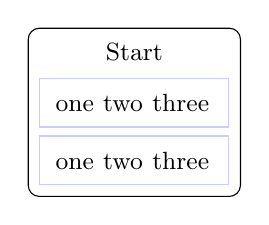
\begin{tikzpicture}
    \node (a) {\small Start};
    \step{a}{b}
    \step{b}{c}
    \begin{pgfonlayer}{background}
      \draw[rounded corners] ($(current bounding box.south west)-(4pt,4pt)$)
        rectangle ($(current bounding box.north east)+(4pt,2pt)$);
    \end{pgfonlayer}
  \end{tikzpicture}
  \end{center}}}
\xdef\SketchSize{\the\wd\sketch/\the\ht\sketch/\the\dp\sketch}
\begin{tikzpicture}
  \node (s) {Base};
  \node[above=1cm of s, scale=0.8, outer sep=0] {\usebox{\sketch}};
\end{tikzpicture}
\gdef\SatexReachedEnd{}
\end{document}
